\section{Auswertung}
\subsection{Drehschieberpumpe}
%Hier 2.1 Beobachtungen, Fragen
%Prinzip einer Drehschieberpumpe



\subsection{Abpumpen kondensierbarer Dämpfe}
%Hier 2.2 Beobachtungen, Fragen,Auswirkung Gasballast
\begin{figure}[h]
	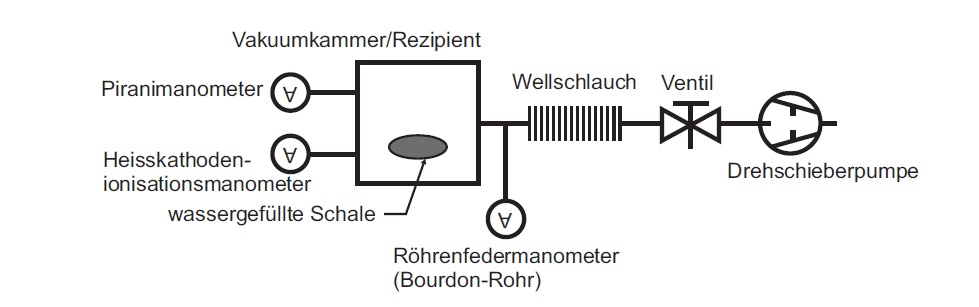
\includegraphics[width=100mm]{Dampf}
	\centering
	\caption{\itshape Blockschaltbild zum Abpumpen kondensierbarer Dämpfe}
	\label{fig:1}
\end{figure}
\noindent

\subsection{Molekular-und Turbomolekularpumpe}
%Hier 2.3, Funktionsweise TMP, mit Gaedestufe, siehe TMP Herstellerangaben hier, kannst einfach die in Anleitung gefragten Werte sonst abschreiben
\begin{figure}[h]
	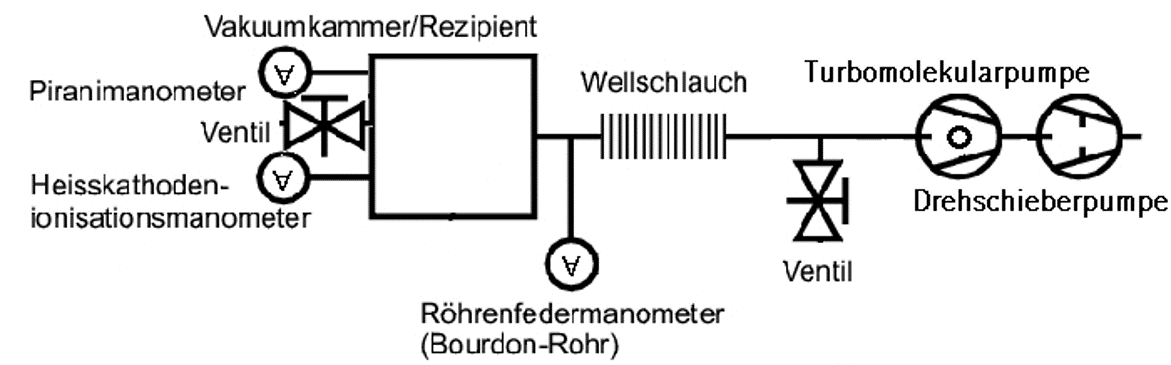
\includegraphics[width=100mm]{TMPmitVorpumpe}
	\centering
	\caption{\itshape Blockschaltbild der Turbomolekularpumpe mit Drehschieberpumpe als Vorpumpe}
	\label{fig:2}
\end{figure}
\noindent

\subsection{Saugvermögen der TMP}
%Hier 2.4, 

\begin{figure}[h]
	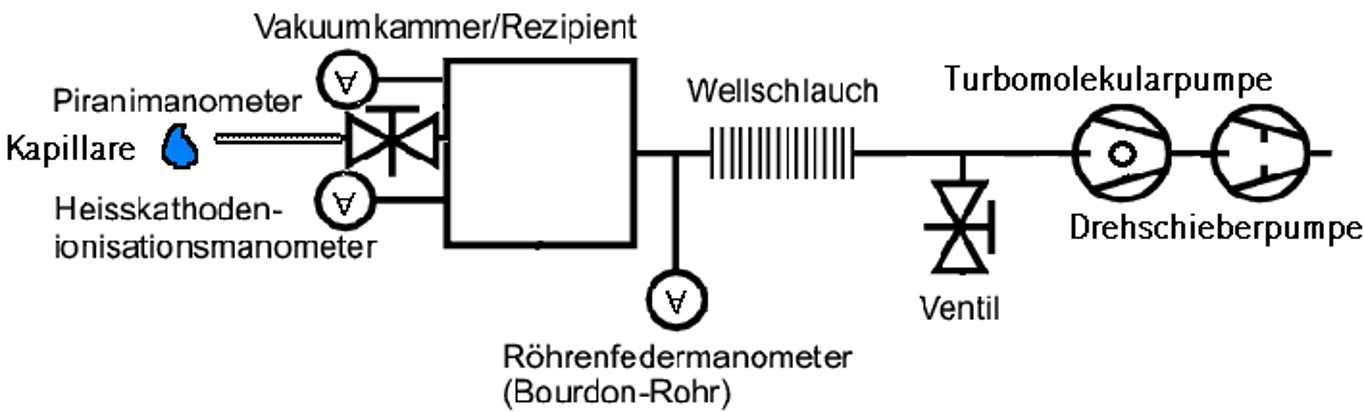
\includegraphics[width=100mm]{Saug}
	\centering
	\caption{\itshape Blockschaltbild Saugvermögen der TMP}
	\label{fig:3}
\end{figure}
\noindent


%\begin{figure}[h]
%	\includegraphics[width=100mm]{SaugvermögenDruck}
%	\centering
%	\caption{\itshape Saugvermögen als Funktion des Logarithmus des Drucks}
%	\label{fig:4}
%\end{figure}
\noindent
\newpage
\subsection{Leitwert von Rohr und Blende}
%Hier 2.5

\begin{figure}[h]
	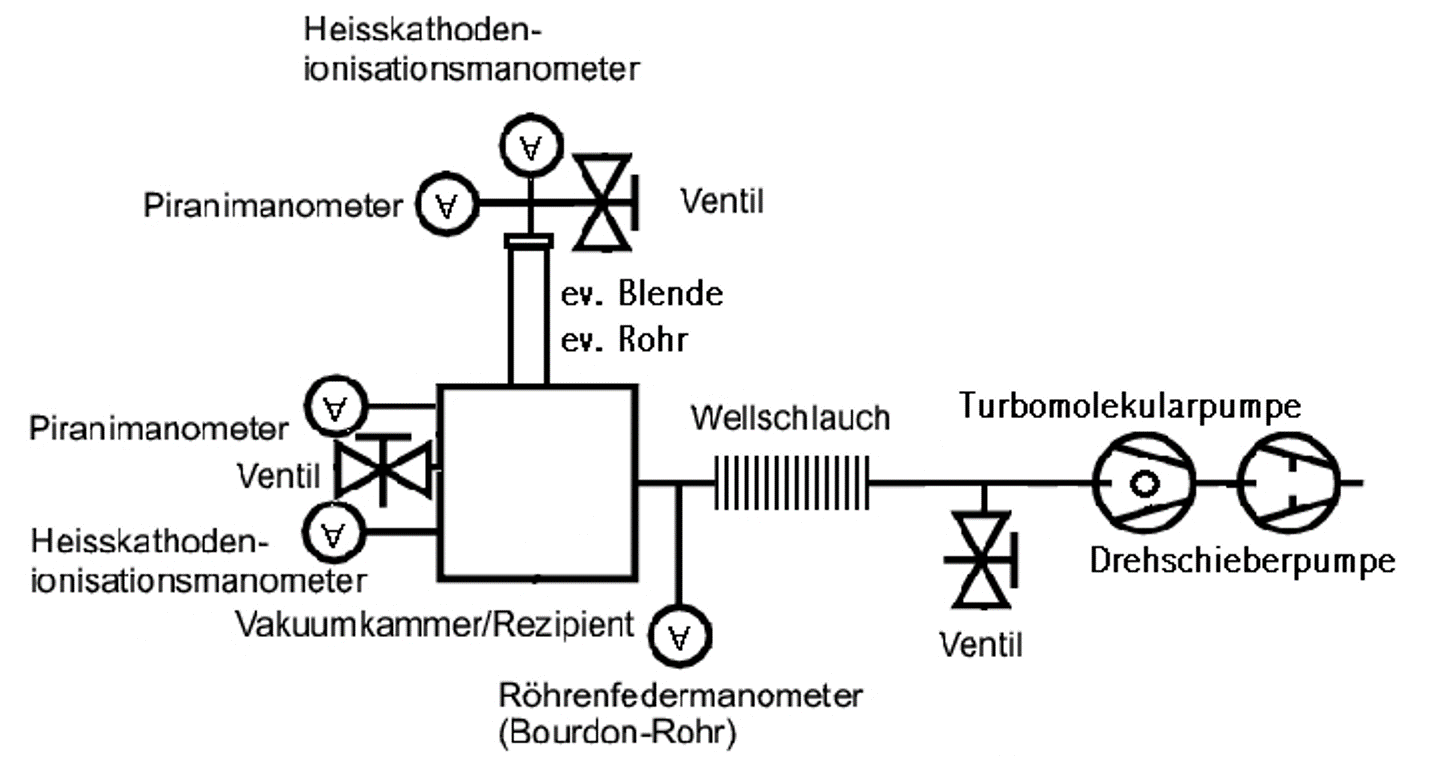
\includegraphics[width=100mm]{LeitwertVonRohrUndBlende}
	\centering
	\caption{\itshape Blockschaltbild Saugvermögen der TMP}
	\label{fig:5}
\end{figure}

%\begin{figure}[h]
%	\includegraphics[width=100mm]{Leitwer1}
%	\centering
%	\caption{\itshape Leitwert von als Funktion des Logarithmus des Drucks}
%	\label{fig:6}
%\end{figure}
\noindent


%\begin{figure}[h]
%	\includegraphics[width=100mm]{Leitwert2}
%	\centering
%	\caption{\itshape Leitwert von als Funktion des Logarithmus des Drucks}
%	\label{fig:7}
%\end{figure}
\noindent



\subsection{Lecksuche}
%Hier 2.6

\begin{figure}[h]
	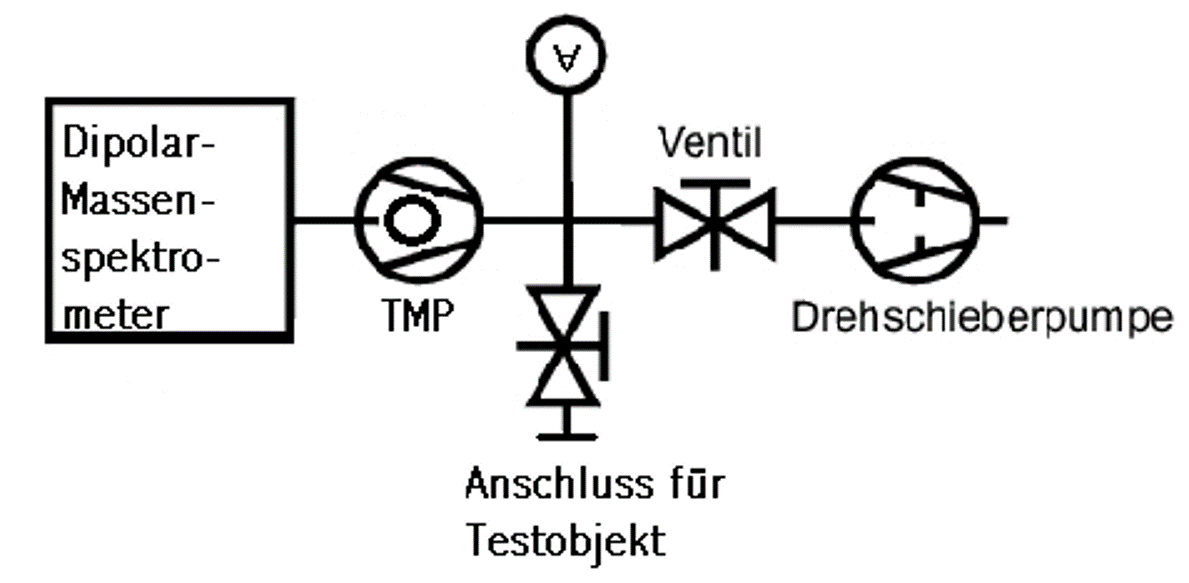
\includegraphics[width=100mm]{GegenstromLecksuche}
	\centering
	\caption{\itshape Blockschaltbild Lecksuche}
	\label{fig:8}
\end{figure}
